% Created 2021-05-06 Thu 12:43
% Intended LaTeX compiler: xelatex
\documentclass[11pt]{article}
\usepackage{graphicx}
\usepackage{grffile}
\usepackage{longtable}
\usepackage{wrapfig}
\usepackage{rotating}
\usepackage[normalem]{ulem}
\usepackage{amsmath}
\usepackage{textcomp}
\usepackage{amssymb}
\usepackage{capt-of}
\usepackage{hyperref}
\usepackage{listings}
\usepackage{color}
\author{Fabio Lima}
\date{\today}
\title{}
\hypersetup{
 pdfauthor={Fabio Lima},
 pdftitle={},
 pdfkeywords={},
 pdfsubject={},
 pdfcreator={Emacs 27.2 (Org mode 9.4.5)}, 
 pdflang={English}}
\begin{document}

\tableofcontents

\section{Radiofármacos}
\label{sec:orgb56c120}

\begin{multicols}{2}

\subsection{História da Radiofarmácia}
\label{sec:org5e64820}

A Radiofarmácia tem seu contexto histórico com o início da utilização dos radio-fármacos em 1905, após a descoberta dos raios X por Wihelm Conrad Roentgen em  seu  laboratório  em  1895.  Além  de  Roentgen,  outros  pesquisadores  contribuíram com destaque para o desenvolvimento da área, dentre eles Marie e Pierre Curie e Henri Becquerel.


Concomitante a essas descobertas, radionuclídeos (nuclídeos que possuem instabilidade no núcleo e que se desintegram espontaneamente emitindo radiação) foram inicialmente utilizados em humanos por Blumgart e Yens em 1927.


Em 14 de junho de 1945, o Oak Ridge National Laboratories anunciou na Revista Science a disponibilidade de radionuclídeos ao setor privado. Posteriormente, o Brookhaven National Laboratories também passou a produzir e comercializar radionu-clídeos, porém esses produtos não possuíam nenhuma garantia de esterilidade e api-rogenicidade. Somente mais tarde, os parâmetros de controle de qualidade foram incluídos, quando a Abbot Laboratories decidiu comprar os laboratórios de produção de radionuclídeos supracitados e transformá-los para a produção de radiofármacos, tornando-se o primeiro produtor no mundo. A comercialização do primeiro radio-fármaco, iodo-131, só começou em 1950


Os radiofármacos são medicamentos radioativos utilizados no diagnóstico e tratamento de doenças.

Em 1957, foi anunciado o desenvolvimento do gerador de molibdênio-99/tecnécio-99 meta estável (\(^{99}\)Mo/\(^{99m}\)Tc). Até os dias de hoje, o radionuclídeo \(^{99m}\)Tc, também denominado elemento número 43, é amplamente utilizado na marcação de reagentes liofilizados na rotina da Medicina Nuclear.

\section{Radiação}
\label{sec:org7d428ca}

A  radiação  é  a  propagação  de  energia  sob  várias  formas.  Dependendo  da  quantidade de energia, pode ser classificada em não ionizantes e ionizantes

\subsection{Radiações não ionizantes}
\label{sec:orgc3a5f35}

As radiações não ionizantes são caracterizadas por não possuírem energia suficiente para remover elétrons da eletrosfera do átomo, não ocasionando o processo de ionização da matéria. São classificadas de acordo com o compri-mento de onda: ultravioleta, luz visível, infravermelho, micro-ondas e ondas de rádio  (Figura  \ref{espectro}).  É  importante  ressaltar  que  quanto  menor  o  comprimento  de  onda, maior é a energia da radiação

\begin{figure}[H]
\centering
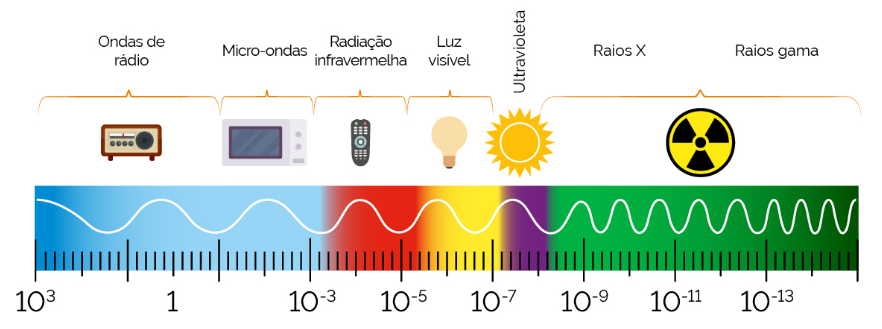
\includegraphics[scale=0.3]{./../QM/espectro.png}
\caption{\label{espectro}Espectro das ondas eletromagnéticas}
\end{figure}


\subsection{Radiações ionizantes}
\label{sec:orga4ed6ba}

As radiações ionizantes possuem energia suficiente para provocar a ionização da matéria, ou seja, são capazes de promover a saída de elétrons da eletrosfera dos átomos, podendo causar modificações na estrutura de moléculas e do DNA (Figura \ref{ionizado}). Estas radiações podem ser corpusculares (partículas alfa e beta) ou ondas eletro-magnéticas (radiação gama).

\begin{figure}[H]
\centering
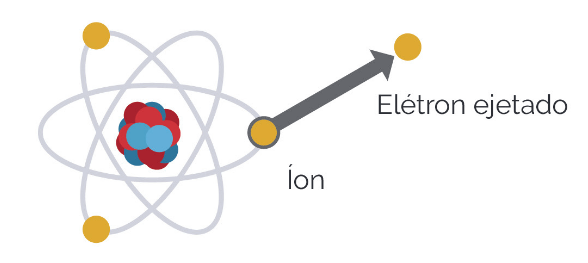
\includegraphics[scale=0.3]{./../QM/ionizado.png}
\caption{\label{ionizado}Processo de ionização.}
\end{figure}



\subsection{Radiação Alfa}
\label{sec:org18a4331}

A partícula alfa (\(\alpha\)) é composta por dois prótons e dois nêutrons (núcleo de hélio), é emitida com alta energia e possui baixo poder de penetração e alto poder ionizante. São emissões típicas de átomos com alto peso atômico. Esse tipo de radiação tem grande importância na medicina para o tratamento de doenças, como o câncer. Exemplos de radionuclídeos emissores de alfa: rádio-223 (\(^{223}\)Ra), urânio-238 (\(^{238}\)U), plutônio-239 (\(^{239}\)Pu).

A radiação beta é subdividida em dois tipos, beta menos (\(\beta ^-\)) e pósitron (\(\beta ^+\)). As emissões do tipo \(\beta ^-\)- possuem a mesma característica dos elétrons atômicos, com a diferença que sua origem se dá no núcleo que possui um número excessivo de nêutrons sendo, portanto, instável. Neste decaimento o nêutron se “transforma” em um elétron (ejetado) e um próton (este permanece no núcleo). Assim como a  radiação  alfa,  elementos  emissores  de  beta  menos  (\(\beta ^-\))  podem  ser  usados  no  tratamento de doenças. Exemplos: lutécio-177 ( \ce{^{177}Lu}),  ítrio-90 (\ce{^{90}Y}).

Outro tipo de emissão beta é o pósitron (\(\beta ^+\)), que consiste na transformação de  um  próton  em  nêutron  e  pósitron  (antielétron),  uma  vez  que  o  núcleo  se  encontra  instável  devido  ao  número  elevado  de  prótons.  Após  sua  emissão  do  núcleo, os pósitrons são quase que instantaneamente aniquilados dando origem a dois fótons com mesma energia (511 keV) e direções opostas. Esse tipo de radiação é utilizado na medicina diagnóstica. Exemplo de radionuclídeos emissores de pósitrons: gálio-68  (\ce{^{68}Ga}), flúor-18 (\ce{^{18}F}).


\subsection{Radiação Gama}
\label{sec:org79f611d}

A radiação gama (\(\gamma\)) é conceituada como ondas eletromagnéticas emitidas do núcleo de um átomo. Apresenta energia superiores e alto poder de penetração, enquanto que os raios X são menos energéticos. Exemplo de radionuclídeos emissores de radiação gama:  \ce{^{99m}Tc}, cobalto-60 (\ce{^{60}Co}).


\section{Poder de penetração da radiação}
\label{sec:orgb1c4542}
As diferentes formas de radiação são emitidas do núcleo com energia e poder de penetração, específicos de cada radionuclídeo; assim são capazes de produzir diferentes efeitos nos seres vivos. A partícula alfa possui grande massa, por isso caminha pouco no meio e uma folha de papel é capaz de barrá-la; e no caso de irradiar o ser vivo, é capaz de penetrar apenas a camada superficial da pele. Por outro lado, a radiação beta, dependendo da energia, pode penetrar milímetros até centímetros, ou seja, é mais penetrante do que a radiação alfa. Por último, a radiação gama que possui a velocidade da luz, pode atravessar blocos de chumbo ou concreto, por possuir alto poder de penetração (Figura \ref{poder}). Com isso, os radio-nuclídeos emissores de alfa e beta podem ser utilizados na terapia de doenças e os emissores de gama, no diagnóstico.

\begin{figure}[H]
\centering
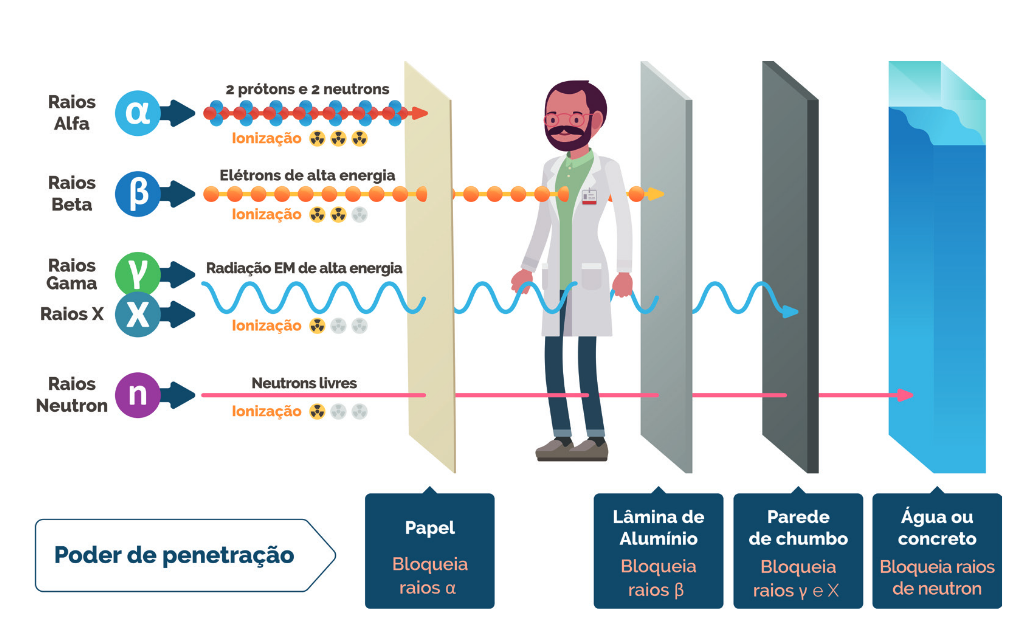
\includegraphics[scale=0.22]{./../QM/poder.png}
\caption{\label{poder}Poder de penetração das radiações.}
\end{figure}



\section{Radionuclídeos e suas origens}
\label{sec:org8e937b8}

Os radionuclídeos podem ser encontrados na natureza, como o  \ce{^238{U}} e o \ce{^{233}Ra}, ou podem ser produzidos artificialmente, de forma direta, em reatores nucleares e cíclotrons, ou de forma indireta, por geradores. O radionuclídeo é um átomo considerado instável em função de seu núcleo pos-suir energia “em excesso”. Essa energia será naturalmente liberada pela emissão de radiação gama, alfa ou beta (processo de desintegração ou decaimento radioativo – Figura \ref{nucle}), com o objetivo de assumir uma condição energética inferior e mais estável; dando origem a novos elementos que podem ser radioativos ou não.


\begin{figure}[H]
\centering
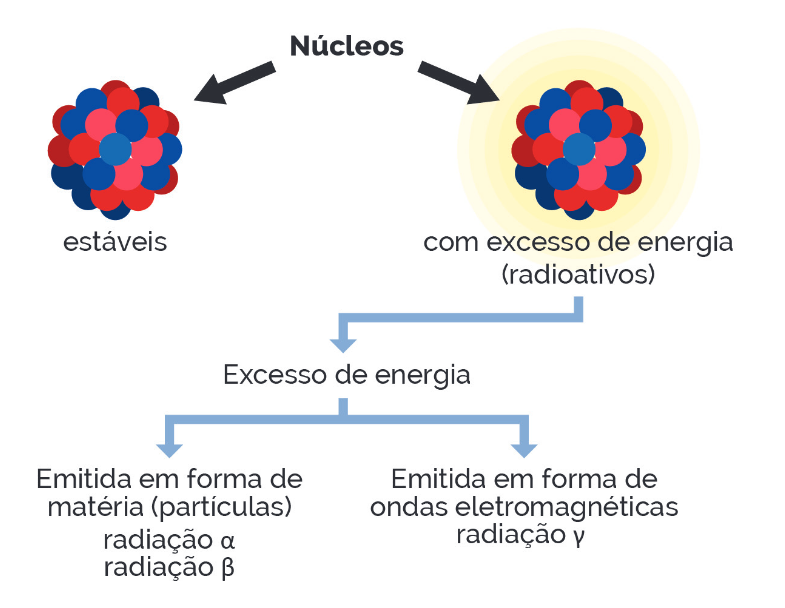
\includegraphics[scale=0.22]{./../QM/nucleo.png}
\caption{\label{nucle}Processo de desintegração do radionuclídeo.}
\end{figure}


\section{Meia-vida física}
\label{sec:org8461112}

Meia-vida física (\(t_{\frac{1}{2}}\)) corresponde ao tempo necessário para a atividade inicial de um elemento radioativo ser reduzida à metade por meio de seu decaimento e consequente emissão de radiação (Figura \ref{meiavida}). A meia-vida de um radionuclídeo pode variar de poucos segundos a vários anos.


Tempo necessário para metade de uma população de átomos de um radionuclídeo decair para outra forma nuclear. A meia-vida é relacionada à constante de decaimento(\(\lambda\)) pela equação:


\begin{equation}
t_{\frac{1}{2}}= \frac{0,693}{\lambda}
\end{equation}

\begin{figure}[H]
\centering
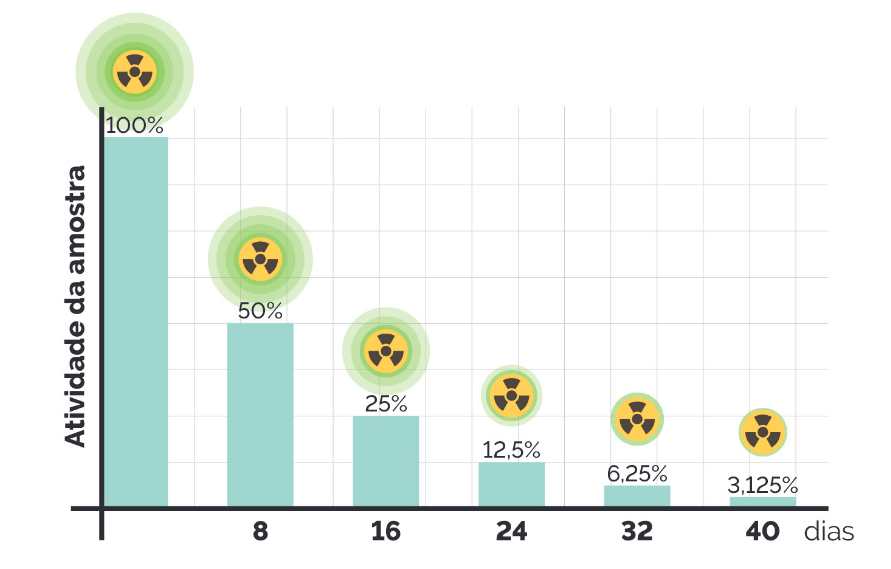
\includegraphics[scale=0.22]{./../QM/meia-vida.png}
\caption{\label{meiavida}Decaimento do  \ce{^{131}I}  pela sua meia-vida física de 8 dias.}
\end{figure}

\subsection{Meia-vida biológica e efetiva}
\label{sec:orgcdc5a52}

A meia-vida biológica representa o tempo necessário para que o organismo excrete 50\% do fármaco. Quando se trata de radiofármacos, é necessário levar em conta também a meia-vida efetiva, que é a soma da meia-vida física e a meia-vida biológica.

A atividade de uma amostra é definida pelo número de desintegrações por segundo do núcleo instável de um radionuclídeo. Dessa forma, é possível mensurar a radioatividade de uma amostra. 

\section{Radiofármaco no Organismo}
\label{sec:orgba007fc}

Para isso, o médico injeta essa solução, que, de acordo com a fisiologia do organismo humano, por meio de afinidades e rejeições com os vários tipos de células, se dirige ao órgão ou região que se quer diagnosticar. A maneira de fazer o diagnóstico em medicina nuclear é diferente da que emprega raios X, em que a radiação atravessa a pessoa sem deixar vestígios e sensibiliza um filme fotográfico. O tecnécio-99m é um emissor de radiação gama. Ao ser injetado no paciente, passa a emitir radiação de dentro do corpo da pessoa, que é captada exteriormente por detectores de radiação.

O médico Celso Dario Ramos, presidente da Sociedade Brasileira de Medicina Nuclear (SBMN), diz que radioisótopos, como o tecnécio-99m, são fundamentais para o diagnóstico de muitas doenças. Outros radioisótopos, como o iodo-131 e o lutécio-177, que também serão produzidos no RMB, possibilitam o tratamento de várias doenças, como o câncer de tiróide e tumores neuroendócrinos. “Com o tecnécio-99m é possível fazer imagens que permitem enxergar o metabolismo celular em tecidos vivos”, explica. “Com os diversos radiofármacos é possível ver a distribuição de um determinado hormônio pelo corpo ou o consumo de glicose em uma região, o que pode revelar a presença e a agressividade de um tumor, por exemplo. Os radiofármacos possibilitam ainda enxergar o funcionamento de órgãos internos, como ossos, pulmões, coração, cérebro, fígado e rins.”

No caso do tecnécio-99m, ele tem uma vantagem adicional: uma meia-vida curta. Meia-vida é o tempo que leva para um elemento radiativo perder (emitir na forma de radiação) metade de seus átomos. “A do urânio-235, por exemplo, é de 700 milhões de anos e a do césio-137, 30,2 anos”, informa Perrotta. “A do iodo-131, outro elemento usado na medicina nuclear e que também será produzido no RMB, é de 8,02 dias e a do tecnécio-99m é de apenas seis horas. Quer dizer, a cada seis horas a intensidade da radiação no corpo da pessoa é reduzida à metade, em dois ou três dias não restará praticamente qualquer intensidade radioativa.”

O fluxo de nêutrons de grande intensidade gerado no RMB servirá para testar combustíveis e materiais usados nos reatores de geração de energia elétrica, como nas centrais nucleares de Angra dos Reis (RJ) e de propulsão, como a que será usada no protótipo do submarino nuclear que a Marinha está desenvolvendo. “O RMB propiciará segurança técnica a esses projetos, garantindo a continuidade no desenvolvimento do conhecimento nuclear do país”, diz Perrotta. “Por fim, ele abrigará um laboratório de uso de feixes de nêutrons em pesquisas de materiais em complemento ao Laboratório Nacional de Luz Síncrotron (LNLS), de Campinas, no interior paulista. Se não avançarmos neste setor, acabaremos à margem do desenvolvimento mundial e ficaremos à mercê do que existe no exterior.”

\end{multicols}


O Tabela \ref{tabfarm} mostra os radiofármacos mais utilizados para tratamentos específicos. Para cada caso há um tempo de exposição e uma dose que varia de fração de segundos a horas.



\begin{table}[htbp]
\caption{\label{tabfarm}Radiofármacos específicos  para tratamento}
\centering
\begin{tabular}{|c|c|}
\hline
\textbf{Radiofármaco} & \textbf{Tratamento}\\
\hline
IODO ( \ce{^{131}I}) & Tumores de tiroíde, fígado e rins\\
\hline
CROMO ( \ce{^{51}Cr}) & Trato de patologias intestinais\\
\hline
GÁLIO ( \ce{^{67}Ga}) & Tumores em tecidos moles.\\
\hline
TECNÉSIO ( \ce{^{99m}Tc}) & Tumores de cérebro, glândulas salivares, coração\\
\hline
GADOLÍNIO ( \ce{^{159}Gd}) & estomâgo, sistema ósseo, fígado, rins, pulmão\\
\hline
\end{tabular}
\end{table}



\begin{figure}[H]
\centering
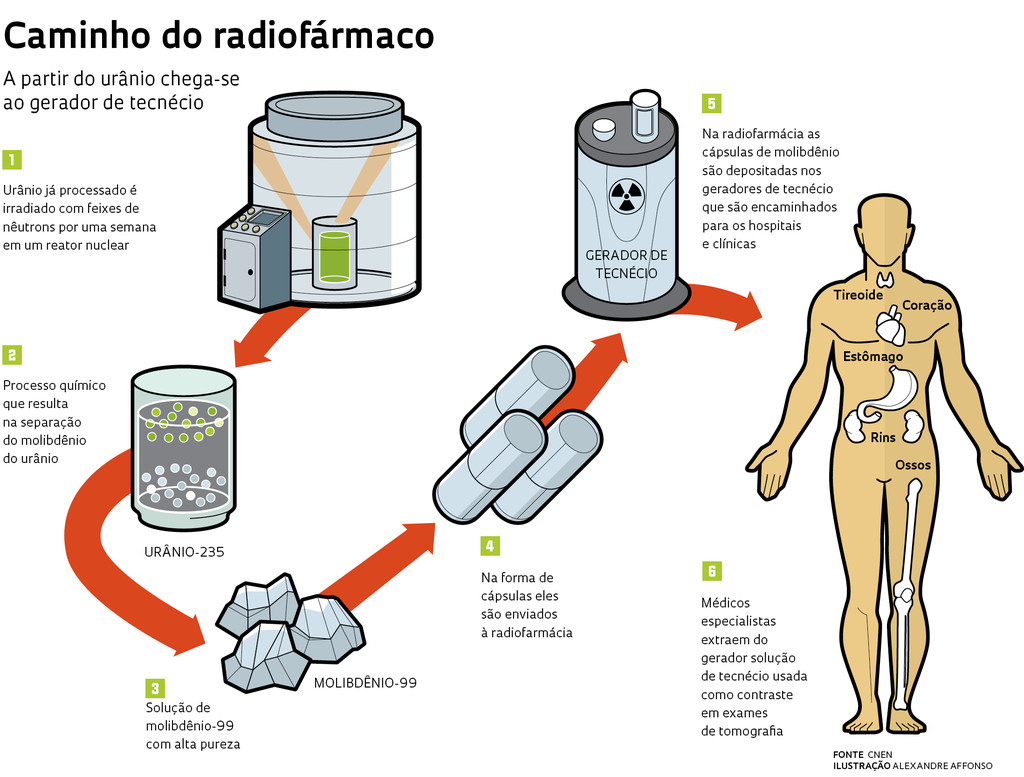
\includegraphics[scale=1.5]{./../QM/caminho.jpg}
\caption{\label{caminho}Representação esquemática do caminho do radiofármaco.}
\end{figure}



\begin{multicols}{2}
\section{Decaimento Radioativo}
\label{sec:orga862efc}

Os decaimentos podem ser de três tipos: \textbf{alfa}, \textbf{beta} e \textbf{gama}. Cada um deles corresponde à uma partícula radioativa diferente, que altera o núcleo do átomo emissor de acordo com suas características.

\textbf{Decaimento alfa:} nela, o núcleo instável emite uma partícula alfa, que é um núcleo de Hélio. Como sabemos da tabela periódica, o Hélio tem dois prótons e dois nêutrons. Assim, o elemento perde 4 de massa, tendo seu número atômico diminuído em 2.

\begin{center}
  \ce{^A_Z X -> ^4_2\(\alpha\) + ^{A-4}_{Z-2}Y} 
\end{center}

\textbf{Decaimento beta:} a partícula beta é um elétron ejetado de um nêutron. Como elétrons não têm massa, ela também não tem. O elemento radioativo tem um nêutron transformado em próton, então aumenta seu número atômico em 1.


\begin{center}
  \ce{^A_Z Q -> ^0_{-1} \(\beta\) + ^{A-0}_{Z+1}R} 
\end{center}

\subsection{Tempo de Meia Vida}
\label{sec:org8b24cfa}

O tempo de meia vida está relacionado à taxa de decaimento de determinada amostra. Ele é o tempo necessário para que metade da quantidade de átomos do elemento radioativo de uma amostra decaia.

Por exemplo, se há 10 átomos radioativos em uma amostra, o tempo de meia vida será o tempo decorrido até que 5 átomos tenham decaído. Depois, dizemos que mais uma meia vida passou quando 2,5 átomos tenham decaído; depois, 1,25, e assim sucessivamente.

\begin{figure}[H]
\centering
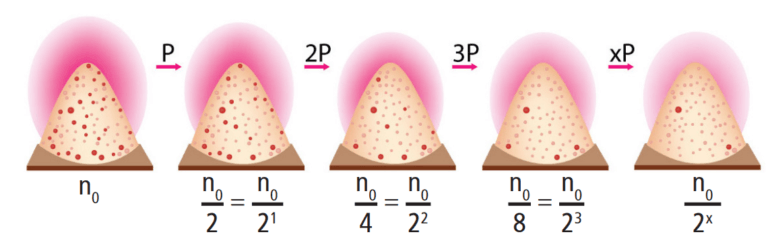
\includegraphics[scale=0.3]{./../QM/tempo-vida.png}
\caption{Decaimento de uma amostra radioativa}
\end{figure}


À medida que o decaimento progride, a quantidade de átomos radioativos diminui pela metade, para cada período P. Assim, a relação matemática fica:

\begin{equation}
 \displaystyle n= \frac{n_0}{2^x} 
\end{equation}

Onde \(n\) é a quantidade final de átomos na amostra. Já \(n_0\) é a quantidade inicial, e \(x\) é o número de períodos de meia vida decorridos. A quantidade de átomos pode ser dada em massa, em mol ou porcentagem sendo todos diretamente proporcionais.

\begin{Box2}{Exemplo}
Vinte gramas de um isótopo radioativo decrescem para cinco gramas em dezesseis anos. A meia-vida desse isótopo é:

a) 4 anos.\\
b) 16 anos.\\
c) 32 anos.\\
d) 10 anos.\\
e) 8 anos.\\
\end{Box2}

\begin{Box2}{Solução}
Os dados apresentados na questão são:

\begin{enumerate}
\item Massa inicial do isótopo: 20 g.
\item Massa final do isótopo: 5 g.
\item Tempo decorrido: 16 anos.
\end{enumerate}


Com base nesses dados, calcula-se quantas vezes a massa reduziu pela metade.

\begin{center}
\begin{tabular}{lllll}
20g & \ch{->[P]} &  \(\rm\displaystyle\frac{20\ g}{2}\)=10g & \ch{->[P]} & \(\rm\displaystyle\frac{10\ g}{2}\)=5 g\\
\end{tabular}
\end{center}

P representa o período que levou para ocorrer essa redução.

Já que a massa passou por duas reduções ao longo dos 16 anos, então quer dizer que a meia-vida desse isótipo é a metade desse tempo.

\begin{align*}
2P = & 16 \text{ anos}\\
P= & \frac{16}{2}\\
P= & \text{8 anos}
\end{align*}
\end{Box2}


Essa relação matemática produz um gráfico com o perfil mostrado abaixo, para o Césio-137. Com ele, podemos saber como o Césio-137 decai a 50\% da amostra inicial ao longo de 35 anos. Assim, sabemos que esse é o tempo de meia vida do Césio-137.


\begin{table}[htbp]
\label{dataCesio}
\centering
\begin{tabular}{rr}
x & y\\
\hline
0 & 20\\
30 & 10\\
60 & 5\\
90 & 2.5\\
120 & 1.25\\
150 & 0.625\\
\end{tabular}
\end{table}

\begin{figure}[H]
\centering
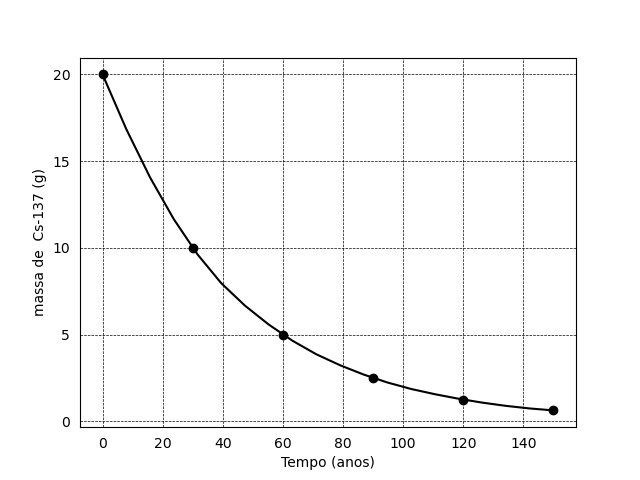
\includegraphics[scale=0.5]{./../QM/decai-curva.png}
\caption{Gráfico sobre o decaimento do Célsio-137}
\end{figure}

\section{Exercícios}
\label{sec:orgc0bed51}

\begin{questions}
\begin{exercise}
Organize o seguinte de acordo com sua capacidade de atuar como escudos de radiação, com o melhor primeiro e o pior por último. Explique sua ordem em termos de como a radiação perde sua energia na matéria.

(a) Um material sólido com baixa densidade composto de átomos de baixa massa.

(b) Um gás composto de átomos de alta massa.

(c) Um gás composto de átomos de baixa massa.

(d) Um sólido com alta densidade composto de átomos de alta massa.

 \blank[width=4.8\linewidth,linespread=1.0]{}
\end{exercise}
\begin{exercise}
Freqüentemente, quando as pessoas têm que contornar derramamentos de materiais radioativos, as vemos vestindo macacões brancos (geralmente um material plástico). De quais tipos de radiação (se houver) você acha que esses trajes protegem o trabalhador e como?

 \blank[width=6.8\linewidth,linespread=1.0]{}
\end{exercise}
\begin{exercise}
Que mudanças ocorrem no número atômico e na massa de um núcleo durante cada um dos seguintes cenários de decaimento?
\begin{choice}
\choice uma partícula \(\alpha\) é emitida
\choice uma partícula \(\beta\) é emitida
\choice radiação \(\gamma\) é emitida
\choice um pósitron é emitido
\choice um elétron é capturado
\end{choice}
\end{exercise}
\begin{exercise}
Tecnécio-99m tem meia-vida de 6,01 horas. Se um paciente que recebeu a injeção de tecnécio-99m é seguro deixar o hospital depois que 75\% da dose diminuiu, quando o paciente pode sair?
\end{exercise}
\begin{exercise}
O iodo que entra no corpo é armazenado na glândula tireóide, de onde é liberado para controlar o crescimento e o metabolismo. A tireóide pode ser fotografada se o iodo-131 for injetado no corpo. Em doses maiores, o I-133 também é usado como meio de tratamento do câncer de tireoide. I-131 tem uma meia-vida de 8,70 dias e decai por \(\beta^-\) emissão.

(a) Escreva uma equação para o decaimento.

(b) Quanto tempo levará para 95,0\% de uma dose de I-131 decair?
\end{exercise}
\end{questions}

\end{multicols}
\end{document}
